\documentclass[a4paper,12pt]{article}
\usepackage{amsmath}
\usepackage{amsfonts}
\usepackage{amssymb}
\usepackage{hyperref}
\usepackage{subfig}
\renewcommand{\figurename}{Fig.}
\renewcommand*{\figureautorefname}{Fig.}
\usepackage{graphicx}

\graphicspath{[./images/]}
\usepackage{float}
\usepackage{multirow}
\usepackage{placeins}
\usepackage{color}
\usepackage{array}
\usepackage{cancel}
\usepackage[margin=1in]{geometry}
%\usepackage[left=1.5in, right=1.5in]{geometry}

\usepackage[nameinlink,noabbrev]{cleveref}
\crefname{equation}{eq.}{eqs.} % force abbreviated forms for equation "names"
\Crefname{equation}{Eq.}{Eqs.}
\crefname{figure}{fig.}{figs.}
\Crefname{Figure}{Fig.}{Figs.}
\usepackage{booktabs} % For prettier tables



%\usepackage{cmbright}
%\renewcommand{\familydefault}{\sfdefault}

\newcommand{\diff}{\mathrm{d}}
\newcommand{\V}[1]{\boldsymbol{#1}}
\newcommand{\B}[1]{\mathbf{#1}}
\newcommand{\myhat}[2]{\hat{#1}_{#2}}
\renewcommand*\arraystretch{1.5}
\renewcommand{\div}[1]{\nabla_{#1} \cdot}
\newcommand{\lapl}{\nabla^2}
\newcommand{\grad}[1]{\nabla_{#1}}
\newcommand{\curl}{\nabla \times}
\newcommand{\Tr}{\mathrm{Tr}}
\newcommand{\op}[1]{\mathcal{#1}}


\newcommand{\T}[1]{\tilde{#1}}
\newcommand{\WT}[1]{\widetilde{#1}}


\newcommand{\yxb}[1]{  {\bf \color{red}{ Bao: #1}} }
\newcommand{\ygq}[1]{  {\bf \color{blue}{ Qin: #1}} }

\DeclareMathAlphabet\mathbfcal{OMS}{cmsy}{b}{n}


\title{Directional Solidification Model for Additive Manufacturing Testbed Problem}
\author{Yigong Qin and Yuanxun Bao}
\date{\today}


\begin{document}

\maketitle




\section{Microscopic model}
We consider the Echebarria model \cite{Tourret2015,Echebarria2010,Plapp2007,Echebarria2004} with frozen temperature approximation, i.e., fixed $G,R$,
\begin{align}
    & T(z,t) = T_0 + G(z-Rt),
\end{align}
where $T_0 = T_m - |m|c_l^0$ and $c_l^0 = c_{\infty}/ k$. 

The compute set of phase-field equations are 
\begin{align}
\tau_{\phi} (\hat{n},z) \frac{\partial \phi}{\partial t} &= W^2_0 \left\{ \div{} [a_s(\hat{n})^2 \grad{} \phi] +  \partial_x \left( |\grad{} \phi|^2 a_s(\hat{n}) \frac{\partial a_s(\hat{n})}{\partial (\partial_x \phi)}  \right)  +
\partial_z \left( |\grad{} \phi|^2 a_s(\hat{n}) \frac{\partial a_s(\hat{n})}{\partial (\partial_z \phi)}  \right)  \right \}  \nonumber \\
& \quad + \phi - \phi^3 - \lambda (1-\phi^2)^2 \left(U + \frac{z-R t}{ l_T} \right),  \label{eq:micro_phi}\\
\tau_U \frac{\partial U}{\partial t} &= \div{} [D_l d(\phi) \grad{} U + \vec{j}_{at}] + [1+(1-k)U]\frac{1}{2}  \frac{\partial \phi}{\partial t}, \label{eq:micro_U}
\end{align}
where 
\begin{align}
U = \frac{1}{1-k} \left( \frac{ c/c_l^0}{(1-\phi)/2 + k(1+\phi)/2} -1\right), \quad d(\phi) = (1-\phi)/2 .
\end{align}
Other parameters and terms are defined as
\begin{align}
    & \tau_{\phi}(\hat{n},z) = \tau_0(a_s(\hat{n}))^2 \left[1-(1-k) \frac{(z-Rt)}{ l_T} \right] \\
	& \tau_U = \frac{1+k}{2} - \frac{1-k}{2}\phi \\
	& \vec{j}_{at} =  \frac{1}{2\sqrt{2}} W_0 [1+(1-k)U] \frac{\nabla \phi}{|\nabla \phi|} \frac{\partial \phi}{\partial t} \\
	& a_{s}(\hat{n}) = (1-3\delta)\left\{1+\frac{4 \delta}{1-3\delta}(\hat{n}_x^4 + \hat{n}_z^4) \right\} \\
    & \hat{n} =  \frac{\nabla \phi}{|\nabla \phi|} \\
    & l_T = \frac{|m|c_{\infty}(1/k-1)}{G} \\
    & \lambda =  \frac{5\sqrt{2}}{8}  \frac{W_0}{d_0} = a_{1} \frac{W_0}{d_0} \\
    & d_0 = \frac{\Gamma}{|m|c_{\infty}(1/k-1)} =   \frac{\gamma T_m/L}{|m|c_{\infty}(1/k-1)}  \\
    & \tau_0 =  \frac{0.6267\lambda W_0^2}{D_l} =  \frac{a_{2}\lambda W_0^2}{D_l}
\end{align}


The boundary conditions are periodic in the $x$-direction and no-flux in the $z$-direction.

\subsection{Non-dimensionalized equations}
We use  the interfacial width $W_0$ as the length scale and $\tau_0$ as the time scale to non-dimensionalize the equations:
\begin{align}
 \left[1-(1-k) \frac{(z- \tilde{R} t)}{ \tilde{l}_T} \right] a_s(\hat{n}^2) \frac{\partial \phi}{\partial t} &= 
  \div{} [a_s(\hat{n})^2 \grad{} \phi] + \nonumber  \\  
 & \partial_x \left( |\grad{} \phi|^2 a_s(\hat{n}) \frac{\partial a_s(\hat{n})}{\partial (\partial_x \phi)}  \right)  + 
\partial_z \left( |\grad{} \phi|^2 a_s(\hat{n}) \frac{\partial a_s(\hat{n})}{\partial (\partial_z \phi)}  \right)   \nonumber \\
& \quad + \phi - \phi^3 - \lambda (1-\phi^2)^2 \left(U + \frac{z-\tilde{R} t}{ \tilde{l}_T} \right) \\
\left(\frac{1+k}{2}-\frac{1-k}{2}\phi \right) \frac{\partial U}{\partial t} &= \div{} [\tilde{D}_l d(\phi) \grad{} U + \vec{j}_{at}] + [1+(1-k)U]\frac{1}{2}  \frac{\partial \phi}{\partial t},
\end{align}
where the non-dimensional parameters are  $\tilde{R} = R\tau_0 / W_0$, $\tilde{D_l} = D_l \tau_0 / W_0^2 = a_{2}\lambda$ and $\tilde{l}_T = l_T / W_0$.

\subsection{Non-linear preconditioned transformation of equations}

\begin{equation}
\varphi(x, y, t)=\tanh \left\{\frac{\psi(x, y, t)}{\sqrt{2}}\right\}
\end{equation}

\begin{align}
 \left[1-(1-k) \frac{(z- \tilde{R} t)}{ \tilde{l}_T} \right] a_s(\hat{n})^2 \frac{\partial \psi}{\partial t} &= 
  \div{} [a_s(\hat{n})^2 \grad{} \psi] - \sqrt{2}a_s(\hat{n})^2\phi|\grad{} \psi|^2 + \nonumber  \\  
 & \partial_x \left( |\grad{} \psi|^2 a_s(\hat{n}) \frac{\partial a_s(\hat{n})}{\partial (\partial_x \psi)}  \right)  + 
\partial_z \left( |\grad{} \psi|^2 a_s(\hat{n}) \frac{\partial a_s(\hat{n})}{\partial (\partial_z \psi)}  \right)   \nonumber \\
& \quad + \phi \sqrt{2} - \lambda (1-\phi^2)\sqrt{2} \left(U + \frac{z-\tilde{R} t}{ \tilde{l}_T} \right) \\
\left(1+k-(1-k)\phi \right) \frac{\partial U}{\partial t} &= \div{} [\tilde{D}_l (1-\phi) \grad{} U + \vec{j}_{at}] + [1+(1-k)U]\frac{1-\phi^{2}}{\sqrt{2}}  \frac{\partial \psi}{\partial t},
\end{align}

\begin{align}
	& \vec{j}_{at} =  [1+(1-k)U]\frac{1-\phi^{2}}{{2}}  \frac{\nabla \phi}{|\nabla \phi|} \frac{\partial \psi}{\partial t} \\
	& a_{s}(\hat{n}) = (1-3\delta)\left\{1+\frac{4 \delta}{1-3\delta}(\hat{n}_x^4 + \hat{n}_z^4) \right\} \\
        & \hat{n} =  \frac{\nabla \phi}{|\nabla \phi|} 
\end{align}



\subsection{Noise}

\subsubsection{Noise added at every time step in $\psi$ equation}
At each grid point (i,j) and each time step we add a random perturbation $\eta\beta_{i,j}\sqrt{\Delta t}$ to the value of $\psi$ at the next time step \cite{Tourret2015}
\begin{equation}
\psi_{i, j}(t+\Delta t)=\psi_{i, j}(t)+\Delta t \frac{\partial \psi_{i, j}}{\partial t}+\eta \beta_{i, j} \sqrt{\Delta t}
\end{equation}

where $\beta_{i,j}$ is a random number generated with a flat distribution in the range [-0.5,0.5], $\Delta$t is the time step, and $\eta$ is the noise amplitude.


\section{Micro model discretization}
\subsection{$\phi$-equation}
We first discretize the $\phi$-equation in \cref{eq:micro_phi}. The challenge is to discretize the anisotropic surface tension term. We will make a few simplications. First, note the anisotropic surface tension can be parametrized by $\theta \equiv \arctan(\phi_y / \phi_x)$, i.e., 
\begin{align}
& a_s(\theta)=  1 + \delta \cos(4 \theta) \\
& a_s'(\theta) = -4 \delta \sin(4\theta) 
\end{align}
By using some trigonometric identities (check), and $\cos(\theta) = \phi_x / |\grad{} \phi|$ and  $\sin(\theta) = \phi_y / |\grad{} \phi|$, we have
\begin{align}
& \cos(4\theta) = 1-8\cos^2(\theta) \sin^2(\theta) = 1- 8 \frac{ \phi_x^2 \phi_z^2 }{|\grad{} \phi|^4} \\
& \sin(4\theta) = 4 \sin(\theta) \cos(\theta) ( \cos^2(\theta) - \sin^2(\theta)) = 4 \frac{(\phi_x^3 \phi_z - \phi_x \phi_z^3 )}{|\grad{} \phi|^4}.
\end{align}
We can also write (see Appendix B of \cite{Tourret2015})
\begin{align}
& \partial_x \left( |\grad{} \psi|^2 a_s(\hat{n}) \frac{\partial a_s(\hat{n})}{\partial (\partial_x \psi)}  \right) = \partial_x (-a'_s(\theta) a_s(\theta) \partial_z \psi ) \\
& \partial_z \left( |\grad{} \psi|^2 a_s(\hat{n}) \frac{\partial a_s(\hat{n})}{\partial (\partial_z \psi)}  \right) = 
\partial_z (a'_s(\theta) a_s(\theta) \partial_x \psi).
\end{align}
Therefore,
\begin{align}
 & \div{} [a_s(\hat{n})^2 \grad{} \psi] +  \partial_x \left( |\grad{} \psi|^2 a_s(\hat{n}) \frac{\partial a_s(\hat{n})}{\partial (\partial_x \psi)}  \right)  +
\partial_z \left( |\grad{} \psi|^2 a_s(\hat{n}) \frac{\partial a_s(\hat{n})}{\partial (\partial_z \psi)}  \right) \nonumber \\
= &  \  \partial_x  \underbrace{ \left[ a_s^2(\theta) \partial_x \psi - a'_s(\theta) a_s(\theta) \partial_z \psi \right]}_{=: F} + 
\partial_z \underbrace{ \left[ a_s^2(\theta) \partial_z \psi + a'_s(\theta) a_s(\theta) \partial_x \psi \right]}_{=: J}  
\label{eq:aniso_surf2}
\end{align}

We define $\phi(i,j)$ on the cell nodes. Therefore, \cref{eq:aniso_surf2} is discretized as
\begin{equation}
\frac{F(i+1/2, j) - F(i-1/2,j)}{\Delta x} + \frac{J(i,j+1/2)-J(i,j-1/2)}{\Delta z}
\end{equation}
Note $F,J$ are defined on cell edges. For example, to evaluate $F(i+\frac{1}{2},j)$, we need to evaluate
\begin{align}
& a_s(\theta) \bigg|_{i+1/2,j} = \left( 1-3\delta + 4\delta  \frac{\phi_x^4 +  \phi_z^4}{|\grad{} \phi|^4} \right)\bigg|_{i+1/2,j} \\
& a'_s(\theta) \bigg|_{i+1/2,j} = -16\delta  \frac{(\phi_x^3 \phi_z- \phi_x \phi_z^3 )}{|\grad{} \phi|^4} \bigg|_{i+1/2,j}\\
& \partial_x \phi \bigg|_{i+1/2,j} = \frac{\phi_{i+1,j}-\phi_{i,j}}{\Delta x} \\
& \partial_z \phi \bigg|_{i+1/2,j}  = \frac{\phi_{i,j+1}+\phi_{i+1,j+1}-\phi_{i,j-1}-\phi_{i+1,j-1}}{4\Delta z} 
\end{align}
Note evaluating $\partial_z \phi |_{i+1/2,j}$ requires averaging nearby cells.  Please work out the details for $F(i-1/2,j)$, $J(i,j+1/2)$ and $J(i,j-1/2)$. Many of them are redundant. I think you only need 
$\partial_x \phi |_{i,j+1/2}$ and $\partial_z \phi |_{i,j+1/2}$.




\subsection{Misorientation}
We denote $\alpha_0$ the misorientation angle, and introduce a rotated coordinate $(\T{x},\T{z})$,
\begin{align}
& \left( 
\begin{array}{c}
\phi_{\T{x}} \\ 
\phi_{\T{z}}
\end{array}
\right)
=
\left[
\begin{array}{cc}
\cos \alpha_{0} & -\sin \alpha_{0} \\
\sin \alpha_{0} & \cos \alpha_{0}
\end{array}
\right]
\left( 
\begin{array}{c}
\phi_{x} \\ 
\phi_{z}
\end{array}
\right) \\
& \cos(4\T{\theta}) = \cos(4(\theta-\alpha_0)) =  1- 8 \frac{ \phi_{\T{x}}^2 \phi_{\T{z}}^2 }{|\WT{\grad{}} \phi|^4} \\
& \sin(4\T{\theta}) = \sin(4(\theta-\alpha_0)) =  4 \frac{(\phi_{\T{x}}^3 \phi_{\T{z}} - \phi_{\T{x}} \phi_{\T{z}}^3 )}{| \WT{\grad{}} \phi|^4} \\
& a_s(\WT{\grad{}} \phi  ) = a_s(\T{\theta} )=  1 + \delta \cos(4(\theta-\alpha_0) ) \\
\end{align}
 We replace $a_s(\grad{} \phi)$ in  \Cref{eq:aniso_surf2} by $a_s(\widetilde{\grad{}} \phi )$\cite{Takaki2014}
 \begin{align}
 \left[1-(1-k) \frac{(z- \tilde{R} t)}{ \tilde{l}_T} \right] a_s(\WT{\grad{}} \phi)^2 \frac{\partial \phi}{\partial t} &= 
  \div{} [\tilde{a}_s(\WT{\grad{}} \phi)^2 \grad{} \phi] + \phi - \phi^3 - \lambda (1-\phi^2)^2 \left(U + \frac{z-\tilde{R} t}{ \tilde{l}_T} \right) \nonumber \\
 & \partial_x \left( |\grad{} \phi|^2 a_s(\WT{\grad{}} \phi) \frac{\partial a_s(\WT{\grad{}} \phi)}{\partial (\partial_x \phi)}  \right)  + 
\partial_z \left( |\grad{} \phi|^2 a_s(\WT{\grad{}} \phi) \frac{\partial a_s(\WT{\grad{}} \phi)}{\partial (\partial_z \phi)}  \right)   \nonumber \\
\end{align}

\begin{figure}[h]
\centering
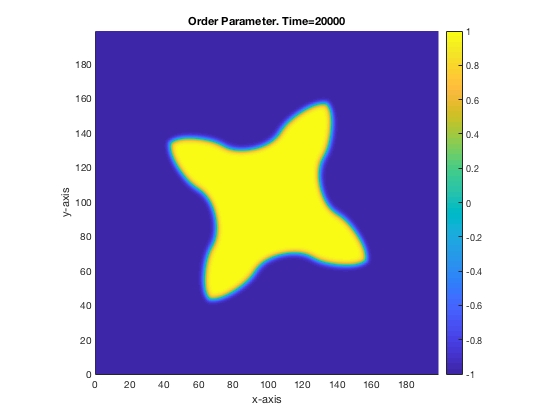
\includegraphics[width=0.5\linewidth]{./figures/misorientation.jpg}
\caption{Misorientation angle $\alpha_0 = \pi/3$}
\end{figure}

\subsection{$U$-equation}
\begin{itemize}
\item A routine that takes in edge-centered vector data and outputs the divergence at cell nodes, i.e.,
\begin{equation}
\div{} \B{u} = \frac{u_{i+1/2,j} - u_{i-1/2,j}}{\Delta x} +  \frac{v_{i, j+1/2} - v_{i,j-1/2}}{\Delta z}
\end{equation}

\item we need the following terms at $(i+1/2,j)$ and $(i,j+1/2)$
\begin{align}
& [(1-\phi) U_x]_{i+1/2,j} = \left( 1- \frac{\phi_{i+1,j} + \phi_{i,j}}{2} \right) \frac{U_{i+1,j}-U_{i,j}}{\Delta x}\\
& [(1-\phi) U_z]_{i,j+1/2} = \left( 1- \frac{\phi_{i,j+1} + \phi_{i,j}}{2} \right) \frac{U_{i,j+1}-U_{i,j}}{\Delta z}\\
\end{align}

\item Similarly, for the anti-trapping flux $\vec{j}_{at}$, we need
\begin{align}
& \left[ [1+(1-k)U]  \frac{\phi_x}{ |\grad{} \phi | } \frac{\partial \psi}{\partial t}  \right]_{i+1/2,j} = \nonumber \\
&  \frac{1}{2}\left[[1+(1-k)U_{i+1,j}]\partial_t\psi_{i+1,j}+[1+(1-k)U_{i,j}]\partial_t\psi_{i,j}\right]  \frac{\phi_x}{ |\grad{} \phi | }\bigg|_{i+1/2,j}  \\
& \left[ [1+(1-k)U]  \frac{\phi_y}{ |\grad{} \phi | } \frac{\partial \psi}{\partial t}  \right]_{i,j+1/2} = \nonumber \\ 
& \frac{1}{2}\left[[1+(1-k)U_{i,j+1}]\partial_t\psi_{i,j+1}+[1+(1-k)U_{i,j}]\partial_t\psi_{i,j}\right]  \frac{\phi_x}{ |\grad{} \phi | }\bigg|_{i,+1/2j}  
\end{align}
\end{itemize}

\section{Implementation}


\subsection{Divide-by-zero treatment}
On page 66 of \cite{Provatas2010}, whenever $|\grad{}\phi(i,j)|^{2} \leq \epsilon $, say $\epsilon = 10^{-8}$, we just set
\begin{align*}
a_s(\hat{n}) &= 1-3\delta, \\
a'_s(\hat{n}) &= 0.
\end{align*}
In \cite{Karma1998}, Karma explained the need for $a_s(\hat{n})$ in the definition $\tau_{\phi}$ on the LHS of \cref{eq:micro_phi} because it is related to the correct kinetics in the Stefan problem. Fortunately this term is never zero so it is safe to divide. 


\subsection{Initial condition}
\subsubsection{Initial condition for $\phi$}
Planar interface perturbed with sinusoidal bumps:
\begin{equation}
\phi(x,z,t=0) = - \tanh \left( \frac{z - z_0 - A_0\sin(2n\pi x /L_x  ) }{W_0}  \right),
\end{equation}
where $z_0$ is the initial height, $A_0$ is the amplitude to initial perturbation, and $n$ is the number of  sinusoidal bumps.  
\subsubsection{Initial condition for U}
As suggested in \cite{Takaki2014}, to avoid confusion, the frozen temperature approximation is:
\begin{align}
    & T(z,t) = T^e + G(z-Rt),
\end{align}
where $T^e$ is the temperature at z=0 and y=0.
And the dimensionless supersaturation, U, is defined as

\begin{equation}
U=\frac{c_{l}-c_{l}^{e}}{c_{l}^{e}-c_{s}^{e}}=\frac{1}{1-k} \left( \frac{ c/c_l^e}{(1-\phi)/2 + k(1+\phi)/2} -1\right)
\end{equation}
$c_l^e$ and $c_s^e$ are the equilibrium concentrations of the liquid and solid at $T^e$, respectively. $c_s^e=kc_l^e$.
The relation between $T^e$ and $c_l^e$ is:
\begin{equation}
c_l^e = \frac{T_m-T^{e}}{m}
\end{equation}
$T_m$ is the melting temperature of the pure material.

\subsection{Moving domain}




\begin{table}
\centering
\caption{Physical and simulation parameters for SCN \cite{Tourret2015}.}
\begin{tabular}{l l c c }
\toprule
symbol & meaning & values & units \\
\midrule
$c_{\infty}$ & nominal solute concentration &  0.4 & K \\
$m$ &liquidus slope &  -3.02 & K \\
$k$ & interface solute partition coefficient & 0.1 &\\
$D_l$ & solute diffusion coefficient &  $1.27\times 10^{3}$  & ${\mu\text{m}}^2/\text{s}$ \\
$\delta$ & strength of the surface tension anisotropy  &  0.007  &\\
$\Gamma$ & Gibbs-Thompson coefficient & $6.4\times 10^{-8}$ & Km \\
$G$ & thermal gradient & 100-300 & $\text{K} / \text{cm}$ \\
$R$ & pulling speed &  25 & $\mu \text{m} / \text{s}$ \\
$l_T$ & thermal length &  0.362-10.9  & mm \\
$l_D$ & length &  50.8  & $\mu$m \\
$d_0$ & capillary length & $ 5.89\times10^{-3}$  & $\mu$m \\
$W_0$ & interface thickness  & 113.25 & $d_0$ \\
$\Delta x$ & mesh size & 1.5 & $W_0$ \\
\bottomrule
\end{tabular}\label{tab:Tourret}

\end{table}



\section{Simulation results}

 \begin{figure}[!ht]
     \subfloat[$U_0= - 1$\label{subfig-1:phi}]{%
       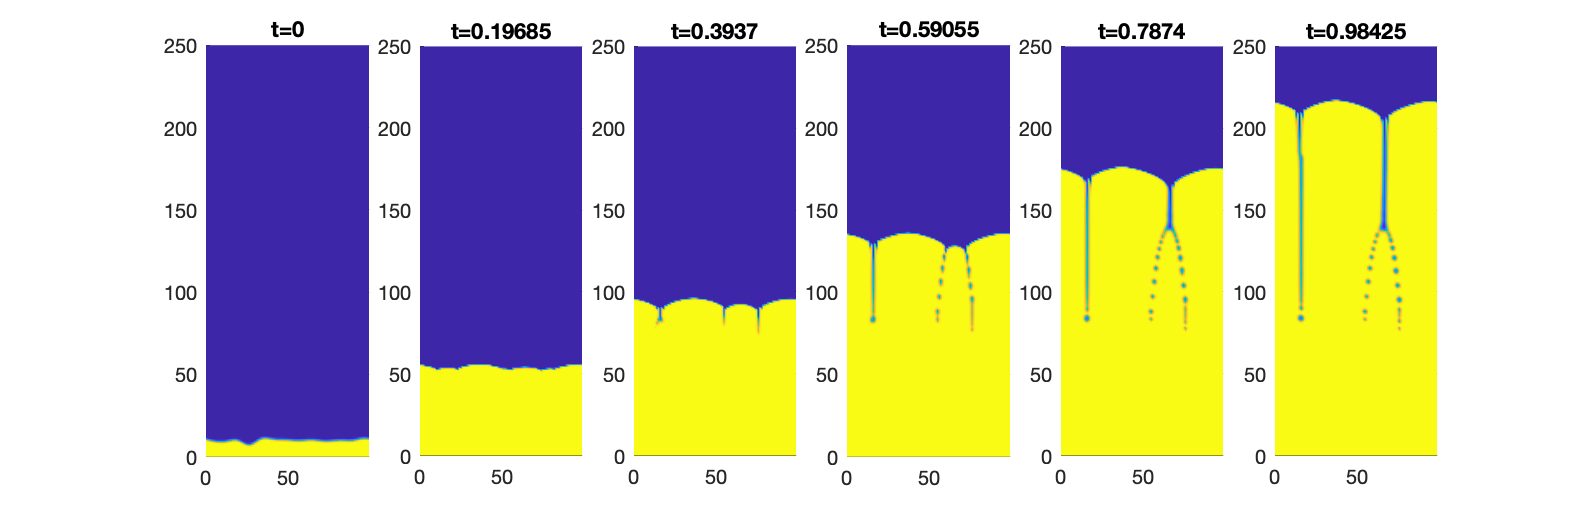
\includegraphics[width=0.5\textwidth]{./figures/U1.png}
     }
     \hfill
     \subfloat[$U_0= - 0.55$\label{subfig-2:c/cinf}]{%
       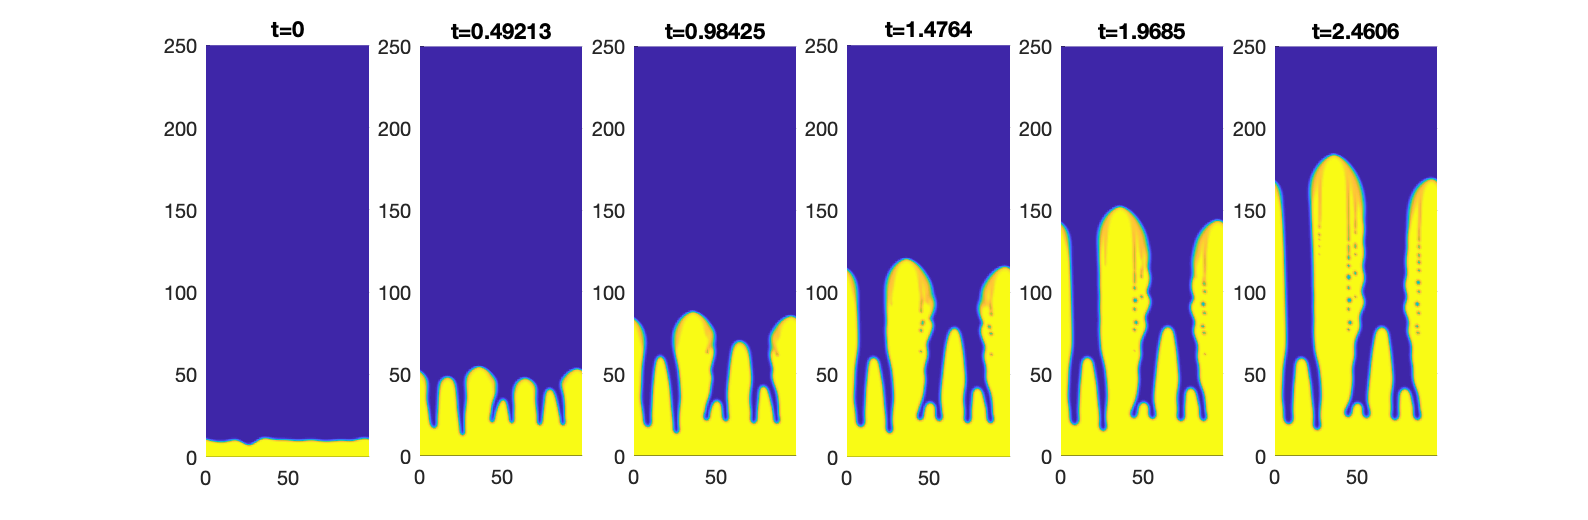
\includegraphics[width=0.5\textwidth]{./figures/U0p55.png}
     }
      \hfill
     \subfloat[$U_0= - 0.3$\label{subfig-2:c/cinf}]{%
       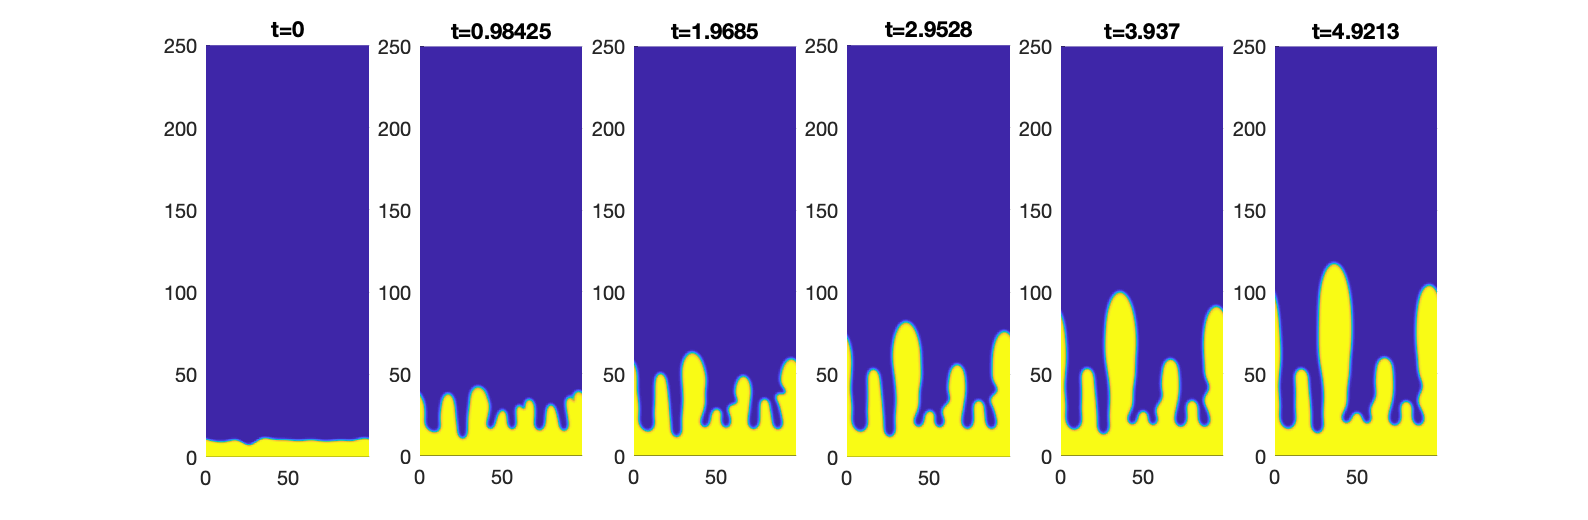
\includegraphics[width=0.5\textwidth]{./figures/Up3.png}
     }     
      \hfill
     \subfloat[$U_0= 0$\label{subfig-2:c/cinf}]{%
       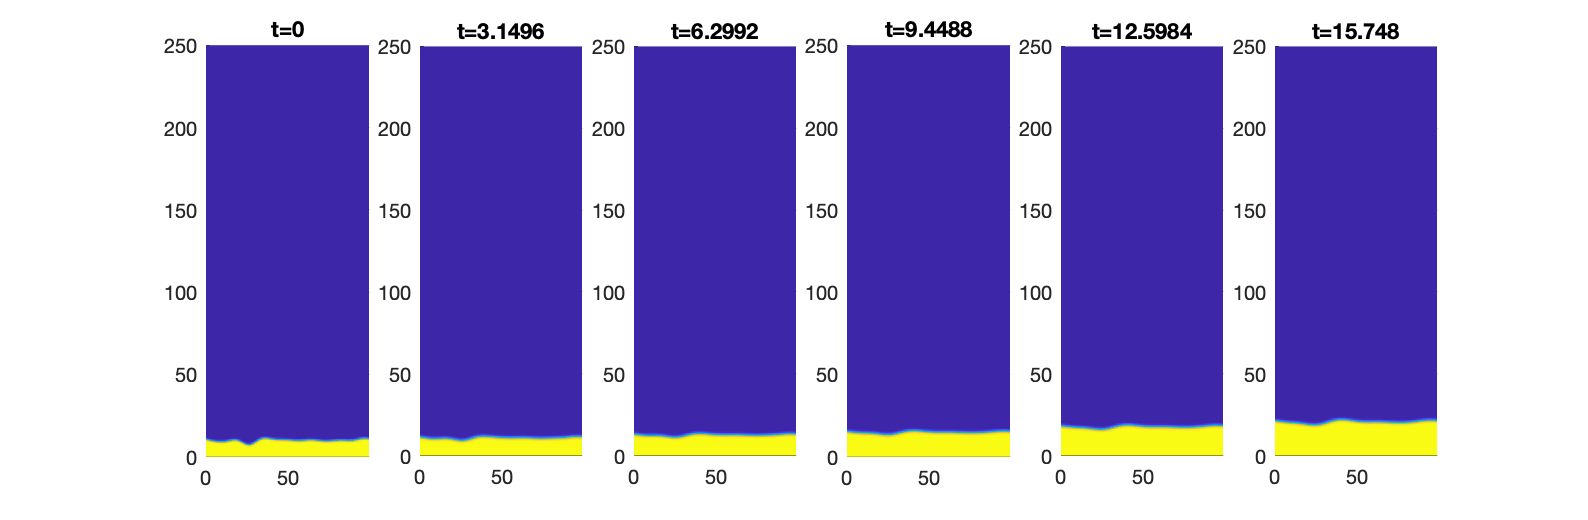
\includegraphics[width=0.5\textwidth]{./figures/U0.png}
     }     
          
     
     \caption{Growth of SCN alloy with same initial perturbations in $\phi$ but different initial value of U. No noise, parameters summarized in Table 1.}
     \label{fig:Ech}
   \end{figure}

\subsection{convergence}
\begin{figure}[h]
\centering
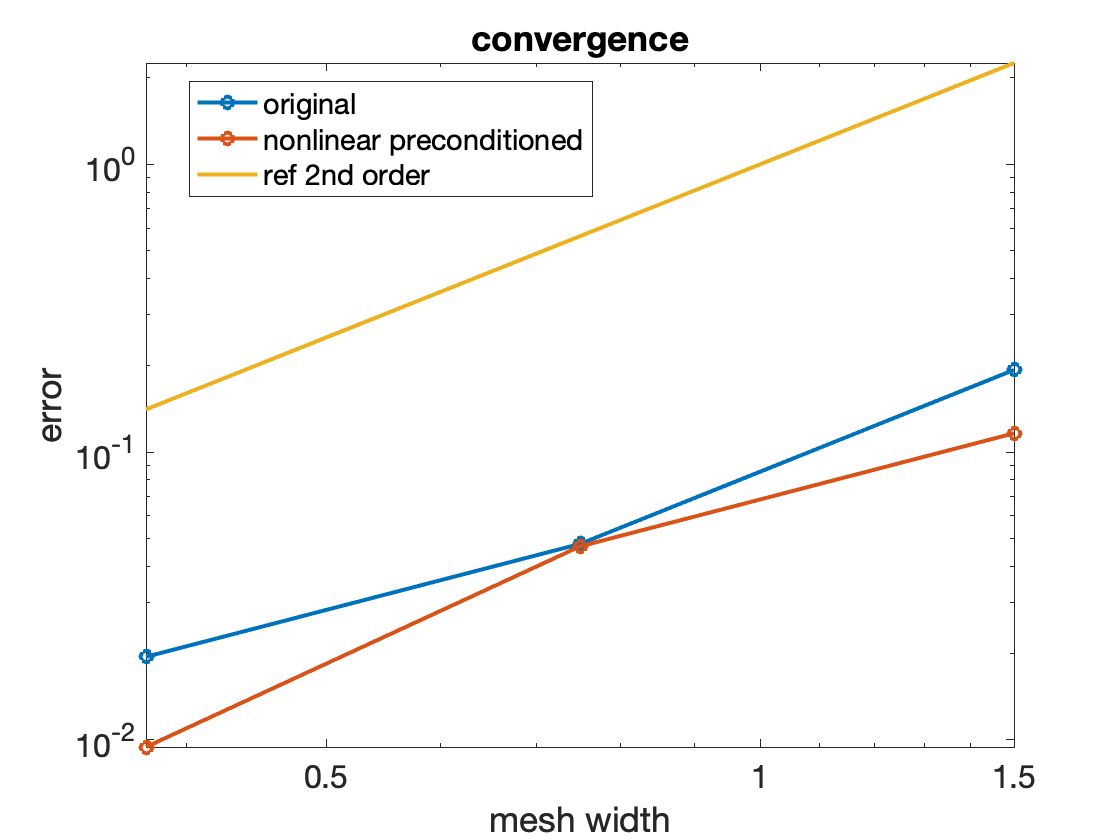
\includegraphics[width=0.5\linewidth]{./figures/preconditioner.png}
\caption{Average error with and without preconditioner}
\end{figure}
   
\subsection{noise model}

\begin{table}
\centering
\caption{Physical parameters for Al-Cu \cite{Takaki2014}.}
\begin{tabular}{l l c c }
\toprule
symbol & meaning & values & units \\
\midrule
$T_m$ & melting temperature of pure Al & 933.25  & K \\
$T^e$ & reference temperature at z=0 and t=0 & 931.20  & K \\
$c_l^e$ & reference equilibrium liquid concentration at $T^e$ & 0.00331  & at. frac. \\
$U_0$ & initial value of U & -0.3  &\\
$c_{\infty}$ & nominal solute concentration &  0.00245 & at. frac. \\
$m$ &liquidus slope &  -620 & K/at. frac. \\
$k$ & interface solute partition coefficient & 0.14 &\\
$D_l$ & solute diffusion coefficient &  $3\times 10^{3}$  & ${\mu\text{m}}^2/\text{s}$ \\
$\delta$ & strength of the surface tension anisotropy  &  0.02  &\\
$\Gamma$ & Gibbs-Thompson coefficient & $2.4\times 10^{-7}$ & Km \\
$G$ & thermal gradient & 200 & $\text{K} / \text{cm}$ \\
$R$ & pulling speed &  50 & $\mu \text{m} / \text{s}$ \\
$d_0$ & capillary length & $ 2.572\times10^{-2}$  & $\mu$m \\
$W_0$ & interface thickness  & 36.45 & $d_0$ \\
$\Delta x$ & mesh size & 1.5 & $W_0$ \\
\bottomrule
\end{tabular}\label{tab:Takaki}

\end{table}

 \begin{figure}[!ht]
 \centering
     \subfloat[My result\label{subfig-1:phi}]{%
       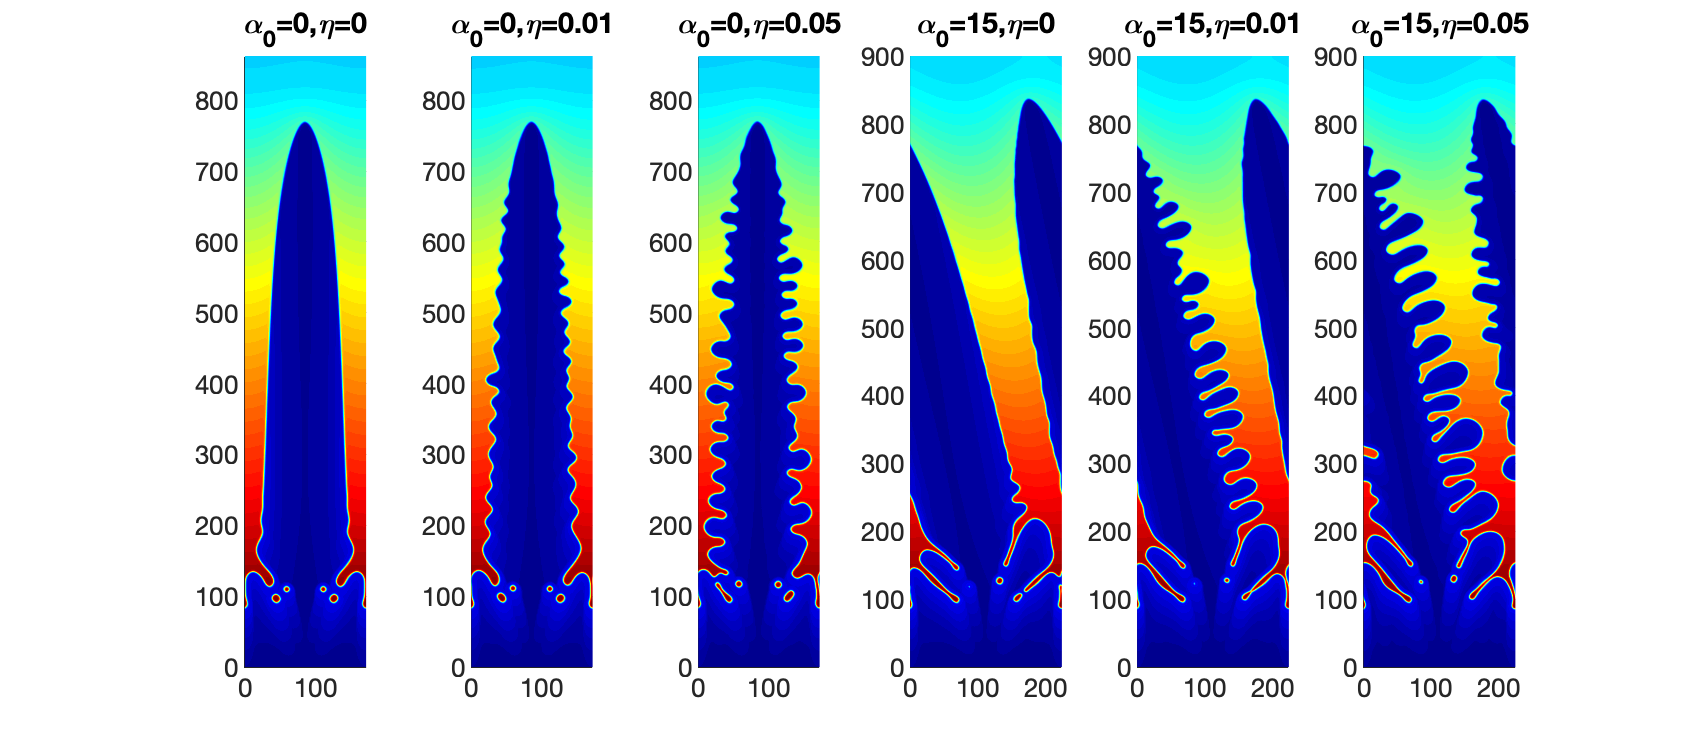
\includegraphics[width=1\textwidth]{./figures/Takaki_noise_level.png}
     }
     \hfill
     \subfloat[Fig. 3(a) of the reference \cite{Takaki2014}\label{subfig-2:c/cinf}]{%
       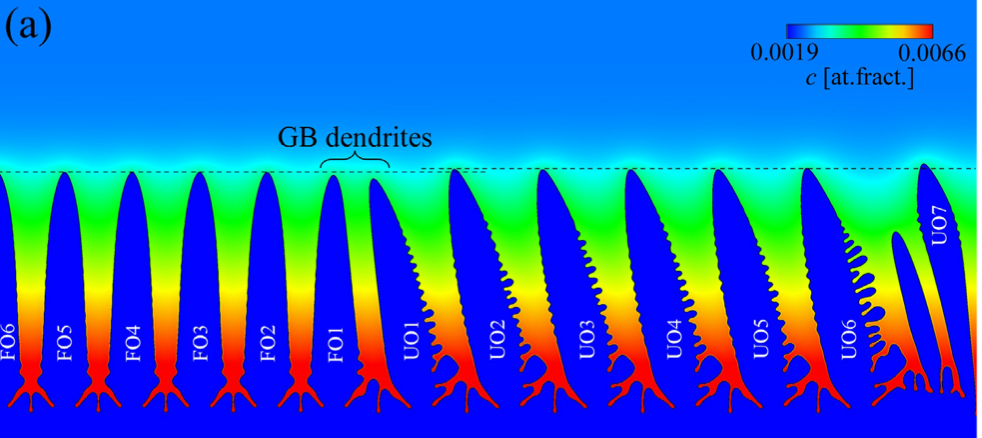
\includegraphics[width=0.7\textwidth]{./figures/TakakiFig3a.png}
     }     
     
     \caption{(a) Dendrite morphologies and concentration distributions with different misorientation angle $\alpha_0$ and noise level $\eta$. Use the same physical parameters of Al-Cu in \cite{Takaki2014}(b) Comparison with the reference \cite{Takaki2014}}
     \label{fig:Ech}
   \end{figure}
\bibliographystyle{unsrt}
\bibliography{Directional-Solidification.bib}


%%%%%%%%%%%%%%%%%%%%%%%%%%%%%%%%%%%%%%%%%%%%%%%

\end{document}